\chapter{Evalutation}

This chapter covers the evaluation of the final product, the process model and what the team learned in this course.

\section{Problems and Difficulties}
	First problem that the group met, was to not deal with incompatible licenses. This was quite hard because much is licensed as GPL 1 or 2 and are not compatible with Apache 2. \\

	The second problem was the decision to write the protocol or use a middleware on a computer.

	The last problem was to get the protocol to work.

\section{Interaction with the customer}
	The communication with the customer was great. A regular meeting was held every Friday, and the customer had an insight to the projects repositories, so the customer allways knew what was going on. 

\section{Usage of workhours}
	The group decided from the beginning that every member should work approximately 20 hours every week.
	In Table ~\ref{table:workhours} it is listed the total workhours for the group on every iteration.

	\begin{table}[H]
	\caption{Iterations and time spent}
	\centering
	\label{table:workhours}
	\begin{tabular}{|l|l|}
		\hline
			{\bf Iteration} & {\bf Hours}\\
		\hline
			Iteration 1 (Week 6-7) & 186 hours\\
		\hline
			Iteration 2 (Week 8-9) & 257 hours\\
		\hline
			Iteration 3 (Week 10-11) & 233 hours\\
		\hline
			Iteration 4 (Week 12-13) & 129 hours\\
		\hline
			Iteration 5 (Week 14-15) & 195 hours\\
		\hline
			Iteration 6 (Week 16-17) & 220 hours\\
		\hline
			Iteration 7 (Week 18-19) & 263 hours\\
		\hline
	\end{tabular}
	\end{table}

	An associated chart diagram of the workhours are shown in Figure ~\ref{fig:workhours}

	\begin{figure}[H]
	\centering
	\captionof{figure}{Workhours in each iteration}
	\label{fig:workhours}
	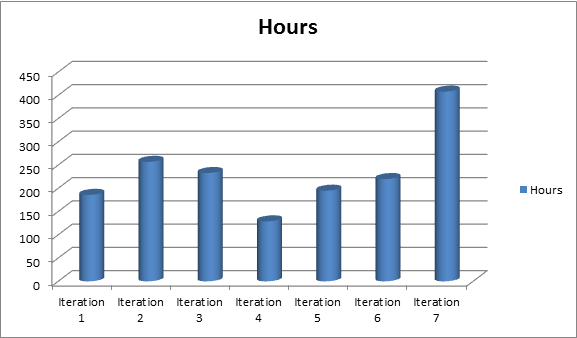
\includegraphics[scale=0.8]{images/workhours_chart2.png}
	\end{figure}

	\section{Process}
	The overall process has been going well. The group have learned to document issues and tasks on the way. This made the process flow steady forward and made it clear and organized. Every member always knew what to do when he or her checked the issue list on Git.

	The communication in the group was also good when the group worked together almost every day and had a group meeting every week. The group could also contact each other via Skype, phone and email.

	\section{The System}
	The $\mu$C Software Store application is almost ready to use. A few changes is still needed to be implemented before it can enter the market. 

	\subsection{Requirements met}
		

	\subsection{Requirement not met}

	\section{Conclusion}